\documentclass[12pt,a4paper]{article}
\usepackage[left=2.54cm, right=2.54cm, top=2cm, bottom=2cm]{geometry}
\usepackage[utf8]{inputenc}
\usepackage{mathtools}
\usepackage{amsmath, amssymb, amsfonts, amsthm}
\usepackage{multicol}
\usepackage{cite}
\usepackage{siunitx}
\usepackage{gensymb}
\usepackage{textcomp}
\usepackage{float}
\usepackage[caption = false]{subfig}
\usepackage{graphicx}
\usepackage{hyperref}
\hypersetup{
    colorlinks=true,
    linkcolor=blue,
    filecolor=magenta,      
    urlcolor=cyan,
}
\urlstyle{same}

%Custom Commands
\newcommand{\git}{{\texttt{git}}}
\newcommand{\github}{{\texttt{Github }}}
\newcommand{\python}{{\texttt{python}}}
\newcommand{\numpy}{{\texttt{numpy}}}
\newcommand{\Anaconda}{{\texttt{Anaconda}}}
\newcommand*\diff{\mathop{}\!\mathrm{d}}
\newcommand*\Diff[1]{\mathop{}\!\mathrm{d^#1}}
\newcommand{\ket}[1]{\left |#1\right \rangle}  
\newcommand{\bra}[1]{\left \langle #1\right |}  
\newcommand{\braket}[2]{\left \langle #1 \vert #2 \right \rangle}


\begin{document}


\title{\textbf{Simulation of Jupiter Trojan Asteroids} \\ \large Computational Physics Final Project}
\author{Chen Ding (cd2209) \\ \small Department of Physics, New York University} 
\date{Dec 16, 2016}
\maketitle

\section{Introduction}

In astronomy, a trojan is a minor planet or moon that shares the orbit of a planet or larger moon, wherein the trojan remains in the same, stable position relative to the larger object. In particular, a trojan remains near one of the two trojan points of stability - designated L4 and L5 - which lie approximately 60$^{\circ}$ ahead of and behind the larger body, respectively. Trojan points make up two of five types of Lagrangian points.

\begin{figure}[H]
\centering
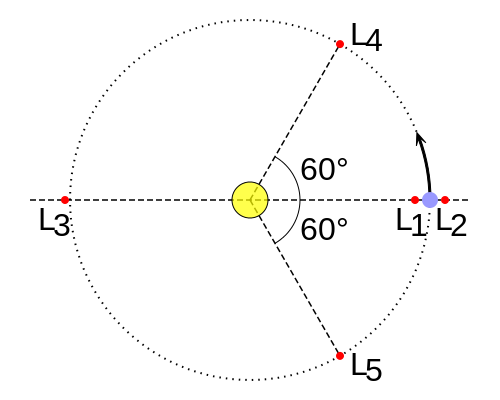
\includegraphics[width=3in]{500px-Lagrange_very_massive.png}
\caption{The trojan points are those labelled L4 and L5, highlighted in red, on the orbital path of the secondary object (blue), around the primary object (yellow).}
\end{figure}

\begin{figure}[H]
\centering
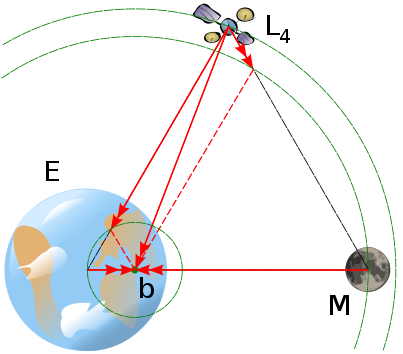
\includegraphics[width=2.5in]{403px-L4_diagram.png}
\caption{Gravitational accelerations at L4 points towards barycenter}
\end{figure}

In this arrangement, the massive star and the smaller planet orbit about their common barycenter. A much smaller mass located at one of the Lagrangian points is subject to a combined gravitational force that acts through this barycenter. Hence the object can orbit around the barycenter with the same orbital period as the planet, and the arrangement can remain stable over time.

The Jupiter trojans account for most known trojans in the Solar System. They are divided into the Greek camp (L4) in front of and the Trojan camp (L5) trailing behind Jupiter in their orbit. More than 6,000 have been found so far and more than a million Jupiter trojans larger than one kilometer are thought to exist, whereas only a few Mars trojans (7) and Neptune trojans (13) have been found to date. The discovery of the first Earth trojan, 2010 TK7, was announced by NASA in 2011.

\begin{figure}[H]
\centering
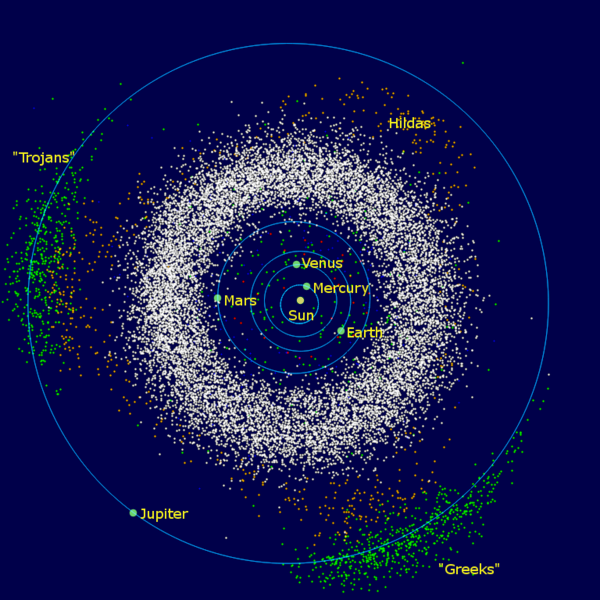
\includegraphics[width=3.5in]{600px-InnerSolarSystem-en.png}
\caption{The Jupiter trojans in front of and behind the planet along its orbital path, the asteroid belt between Mars and Jupiter, and the Hilda asteroids. The Jupiter trojans are divided into two groups: The Greek camp in front of and the Trojan camp trailing behind Jupiter in their orbit.}
\end{figure}

The goal of this project is to simulate the motion of Jupiter Trojan asteroids and make comparison with theory.


\section{Methodology}

\subsection{Units}

Before setting up the equations of motion(EoM) for Sun(S), Jupiter(J) and Asteroid(A), we first need to choose a suitable set of units to make EoMs dimensionless and hence ready for computer simulation:

\begin{itemize}
	\item the unit of length is chosen to be the semi-major axis $a$ of Jupiter.
	\item the unit of time is chosen to be $\displaystyle{\sqrt{\frac{a^3}{GM_S}}}$
\end{itemize}
	
Although none of gravitational constant $G$, mass of Sun $M_S$ or mass of Jupiter $M_J$ are known to great accuracy, the product $GM_S$ and $GM_J$ are known to very high accuracy from astronomical observations. However, only the ratio of masses $\displaystyle{q = \frac{GM_J}{GM_S} \approx 0.0009546}$ enters the EoMs and it is dimensionless.

The eccentricity $e= 0.048498$ of orbit of Jupiter is needed when specifying initial conditions, and it is dimensionless as well.

The period of Jupiter $\displaystyle{\tau = 2\pi \sqrt{\frac{a^3}{G(M_S+M_J)}}}$ becomes $\displaystyle{\tau = 2\pi \sqrt{\frac{1}{1+q}}}$ in this unit set.

\subsection{Equations of Motion}
 
In the set of units we previously specified, the EoMs are simplified to be

\begin{align}
	\ddot{\vec{r_J}} =& - \frac{\vec{r_J}-\vec{r_S}} {{|\vec{r_J}-\vec{r_S}|}^3} \\
	\ddot{\vec{r_A}} =& - \frac{\vec{r_A}-\vec{r_S}} {{|\vec{r_A}-\vec{r_S}|}^3} - q \frac{\vec{r_A}-\vec{r_J}} {{|\vec{r_A}-\vec{r_J}|}^3} \\	
	\ddot{\vec{r_S}} =& \;  q \frac{\vec{r_J}-\vec{r_S}} {{|\vec{r_J}-\vec{r_S}|}^3}
\end{align}

Notice that we assumed the mass of asteroid to be negligibly small so that it will not affect the motion of Jupiter or the Sun. The energy of the whole system is 
\begin{equation}
E = \frac{1}{2} \left({\dot{\vec{v_J}}}^2 +  \frac{1}{q} {\dot{\vec{v_S}}}^2 \right) - \frac{1}{|\vec{r_J}-\vec{r_S}|}
\end{equation}
if we choose the unit of energy as $\displaystyle{\frac{GM_{S}M_{J}}{a}}$.


\subsection{Initial Conditions}
It is convenient to set the barycenter to be at the origin. Let Jupiter starts from aphelion (furthest point in orbit),
\begin{align}
	\vec{r_J} =& (0, \; \frac{1}{1+q} (1+e), \; 0) \\
	\vec{r_S} =& (0, \; -\frac{q}{1+q} (1+e), \; 0) \\
	\dot{\vec{r_J}} =& (-\frac{1}{1+q} \sqrt{\frac{1-e}{1+e}(1+q)}, \; 0, \; 0) \\
	\dot{\vec{r_S}} =& (\frac{q}{1+q} \sqrt{\frac{1-e}{1+e}(1+q)}, \; 0, \; 0).
\end{align}

We put the asteroid at Lagrangian point L5 (trailing behind Jupiter). The Jupiter, Sun, Asteroid form a equilateral triangle. Following from the cosine rule, the distance between asteroid and barycenter
\[
c = (1+e)\sqrt{1-\frac{q}{1+q}+{\left(\frac{q}{1+q}\right)}^2}.
\]
The speed of asteroid (in order to have same angular velocity as Jupiter) is
\[
v =     \sqrt{\frac{1-e}{1+e}(1+q)}   \sqrt{1-\frac{q}{1+q}+{\left(\frac{q}{1+q}\right)}^2}.
\]
The angle of Jupiter-Barycenter-Asteroid
\[
\angle JOA  = \frac{ \frac{q}{1+q}-\frac{1}{2}}{\sqrt{\frac{1-e}{1+e}(1+q)}} = \alpha.
\]

Therefore,
\begin{align}
	\vec{r_A} =& (c \sin{\alpha},  \; c \cos{\alpha}, \; 0) \\
	\dot{\vec{r_A}} =& (-v \cos{\alpha},  \; v \sin{\alpha}, \; 0).
\end{align}

In order to see how asteroid moves under some deviation from Lagrangian point, we give some perturbation to the asteroid by multiplying its speed $v$ (and hence angular velocity) by the perturbation ratio\{1, 1.01, 1.02, 1.03, ...\}.

\subsection{Adaptive RK4}

The next step is to evolve the EoMs. Fourth-order symplectic integrator is a good choice since it conserves the energy of the system. However, the adaptive fourth-order Runge-Kutta method has its own advantages too. It allows us to choose a target for the total accuracy, so that the error would not be large enough to affect the results, nor would it be too small and thus waste time. Also it takes short/long time steps when variables are changing rapidly/slowly, so that it will always reach the accuracy target with little waste. We can always use adaptive RK4 as long as we set a high accuracy target and we check if the energy drift is negligible at the end.

The adaptive RK4 works as follows:

\begin{enumerate}
	\item Use RK4 to evolve one time step $h$, followed by another time step $h$, and get the estimate $x_1$ for $x(t+2h)$.
	\[ x(t+2h) = x_1 + 2ch^5 + \mathcal{O}(h^6). \]
	Here $x$ represents any variable to be evolved.
	
	\item Instead of making two steps of $h$, use RK4 to evolve one time step of $2h$:
	\[ x(t+2h) = x_2 + c{(2h)}^5 + \mathcal{O}(h^6). \]
	$x_2$ is the second estimate of $x(t+2h)$.
	
	\item Therefore, each time step $h$ will introduce an error of 
	\[ \epsilon_x = ch^5  = \frac{1}{30}(x_1-x_2) + \mathcal{O}(h^6). \]
	
	\item The target accuracy for a single time step $h$ is $h \delta$, where,
	\[ \delta = \frac{\textrm{total accuracy target}}{\textrm{total time}}. \]
	
	Compare the error $\epsilon_x$ with target accuracy $h \delta$:
	\[ \rho = \frac{h \delta}{\epsilon_x}.  \]
	
	If $\rho<1$, we decline the time evolution as it introduces an error larger than accuracy target, and we start from $x(t)$ again with reduced time step 
	\[ h' = h {\rho}^{1/4}. \]
	If $\rho>1$, the error is smaller than accuracy target, we accept the time evolution and make $x(t+2h) = x_1$. Also, in the next evolution, we can try a larger time step $h'$ in the hope of going faster. Moreover, in case that $x_1$ and $x_2$ coincide by chance, we limit $h' \leqslant 2h$.
	
	\item It can be realized that
	\[ x(t+2h) = x_1 + 2ch^5 + \mathcal{O}(h^6) = x_1 + \frac{1}{15}(x_1-x_2) + \mathcal{O}(h^6). \]
	If we accept $x_1 + \frac{1}{15}(x_1-x_2)$ instead of $x_1$, the error would be $\mathcal{O}(h^6)$ and the algorithm is accurate to fifth-order instead of fourth order!
	
\end{enumerate}

	
As mentioned earlier, we need to check if the change in total energy is within allowance. Also, we can compare $|\overrightarrow{JS}|$ with the exact value   by solving $M = \psi - e \sin{\psi} $ using Newton-Raphson method, where $M$ is mean anomaly, $\psi$ is eccentric anomaly and $e$ is eccentricity as before.

\begin{figure}[H]
\centering
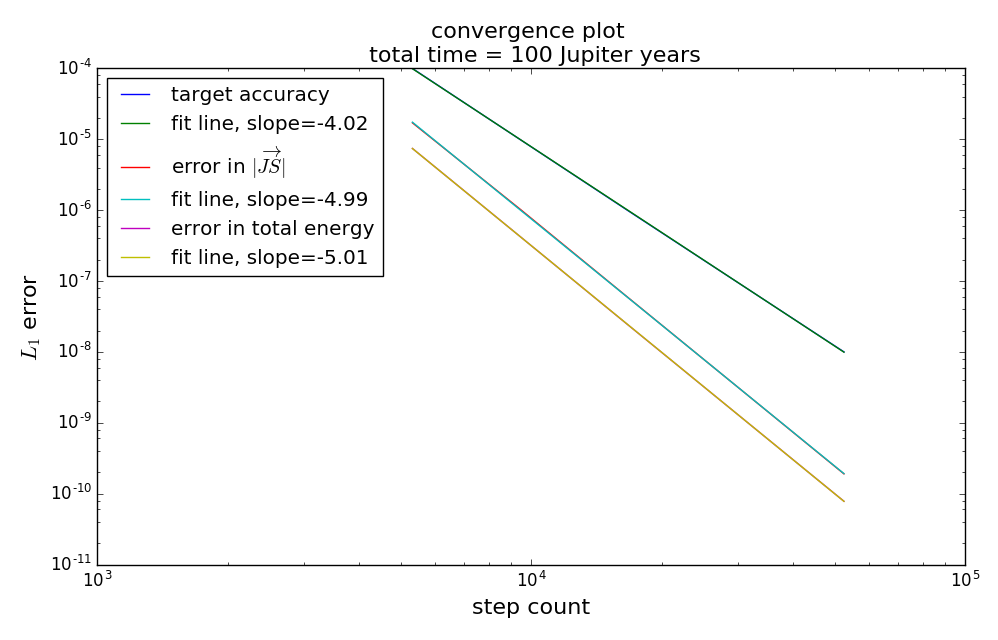
\includegraphics[width=6in]{figure_6_100v_100orbits.png} 
\caption{The convergence plot of error in J-S distance and error in total energy after 100 Jupiter years.}
\label{fig:convergence}
\end{figure}
	
We can see from Figure \ref{fig:convergence} that both the error in $|\overrightarrow{JS}|$ and the change in total energy are negligible after 100 Jupiter years. Thus the use of adaptive RK4 is validated. Also we can see that, we achieved fifth-order accuracy instead of fourth-order, as a result of choosing $x(t+2h) = x_1 + \frac{1}{15}(x_1-x_2)$ instead of $x_1$.


\section{Results and Discussion}

\subsection{Perfect Lagrangian point initial condition, no perturbation}

\begin{figure}[H]
\subfloat[stationary frame]{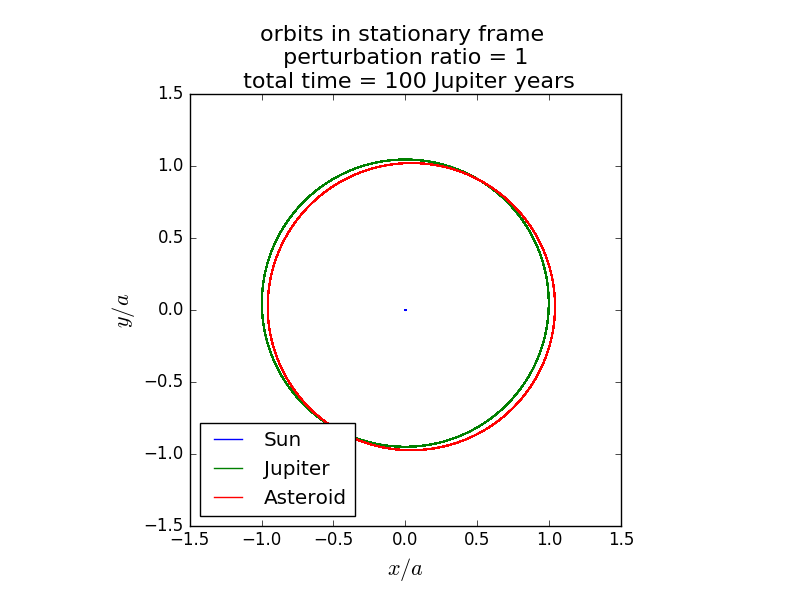
\includegraphics[width = 3.5in]{figure_1_100v_100orbits.png}} \\
\subfloat[constant rotation frame]{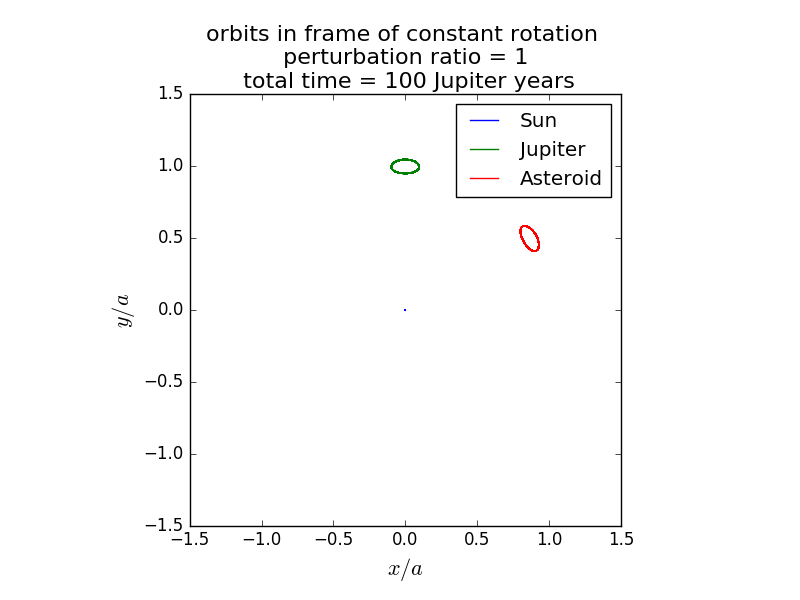
\includegraphics[width = 3.5in]{figure_2_100v_100orbits.png}}
\subfloat[special frame]{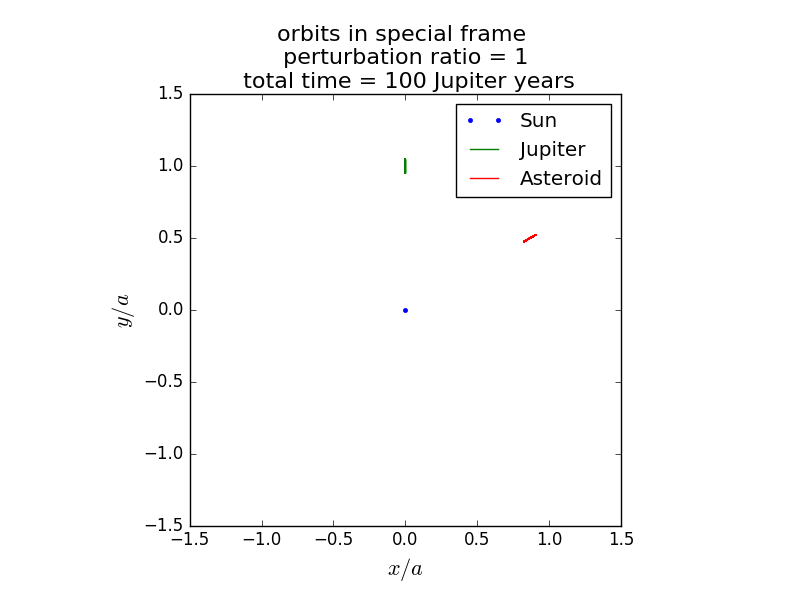
\includegraphics[width = 3.5in]{figure_3_100v_100orbits.png}}
\caption{Orbits of Sun, Jupiter and Trojan asteroid in three different reference frames, in 100 Jupiter years, with perfect Lagrangian point initial condition.}  
\label{fig:figure123_100v_100orbits}
\end{figure}


Figure \ref{fig:figure123_100v_100orbits}(b) shows the orbits in a rotating frame of constant angular frequency that is equal to the average angular frequency of Jupiter. The shape of orbits in this frame is due to the eccentricity of Jupiter orbit. Jupiter is traveling in angular frequency less than average at aphelion, and greater than average at perihelion.

Figure \ref{fig:figure123_100v_100orbits}(c) shows the orbits in a special frame, in which the Sun is fixed at origin, and the Jupiter is fixed in direction. The angular frequency of this rotating frame is varying, giving Euler force in addition to Coriolis force and centrifugal force. However, it has the advantage of showing $\angle JSA$.


\begin{figure}[H]
\centering
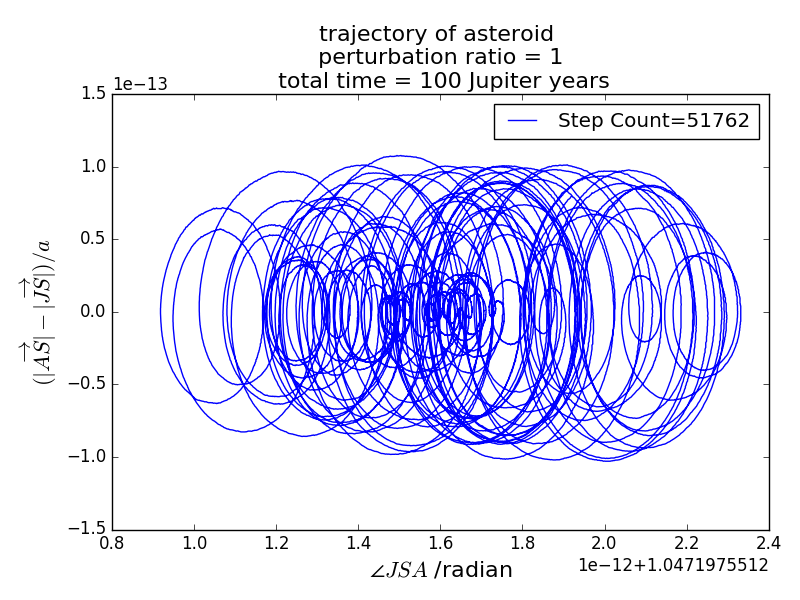
\includegraphics[width = 5 in]{figure_5_100v_100orbits.png}
\caption{Trajectory of Trojan asteroid in 100 Jupiter years, with perfect Lagrangian point initial condition.}  
\label{fig: figure5_100v_100orbits}
\end{figure}


From Figure \ref{fig: figure5_100v_100orbits} we can deduce that, in 100 Jupiter years, the asteroid always make an equilateral triangle with Jupiter and Sun (with extremely small computation error). If an asteroid is given perfect Lagrangian point condition, it will stay at Lagrangian point forever.

\subsection{Including perturbation}

\begin{figure}[H]
\subfloat{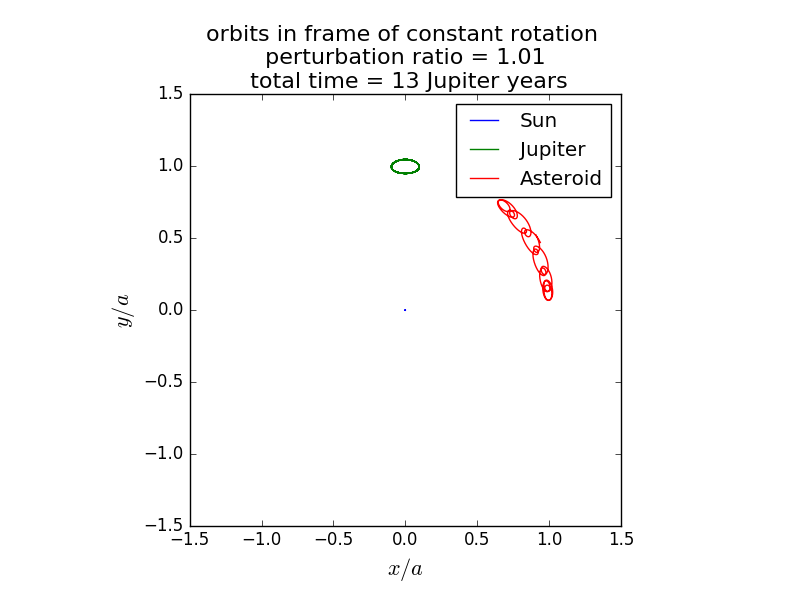
\includegraphics[width = 2.8in]{figure_2_101v_13orbits.png}} 
\subfloat{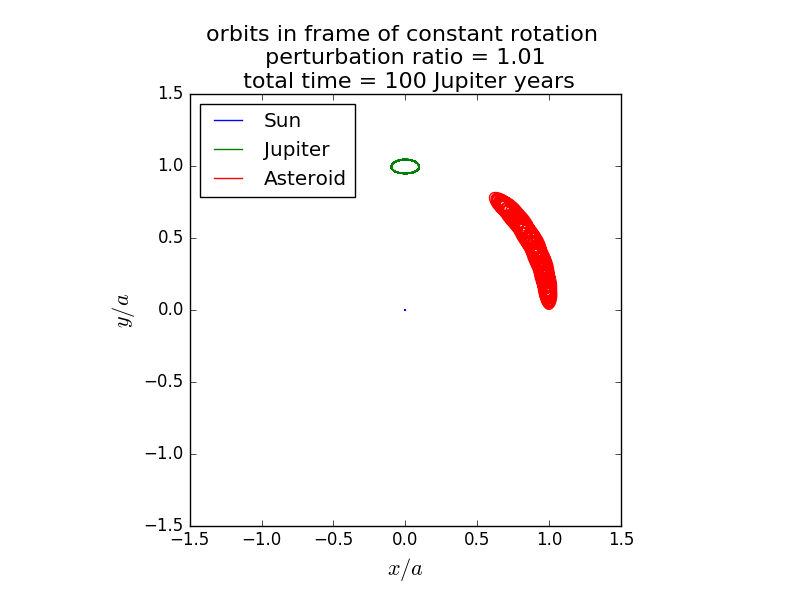
\includegraphics[width = 2.8in]{figure_2_101v_100orbits.png}} \\
\subfloat{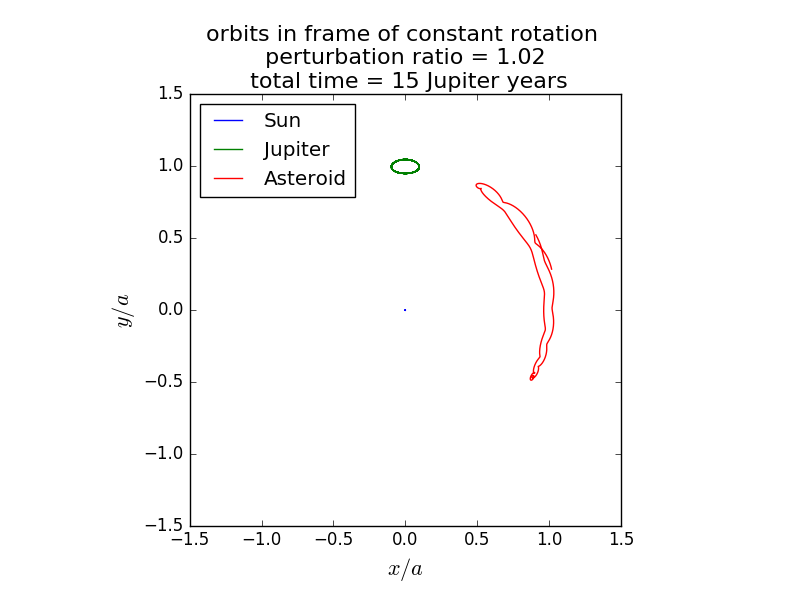
\includegraphics[width = 2.8in]{figure_2_102v_15orbits.png}}
\subfloat{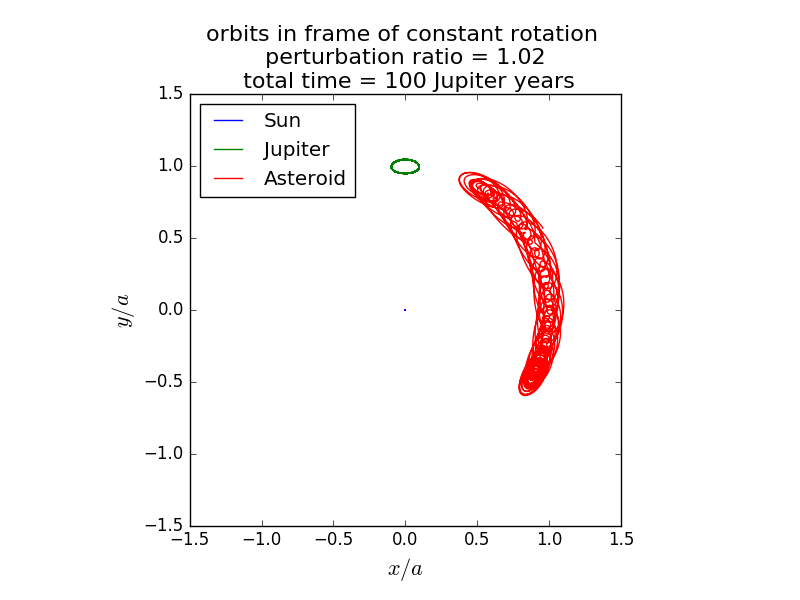
\includegraphics[width = 2.8in]{figure_2_102v_100orbits.png}} \\
\subfloat{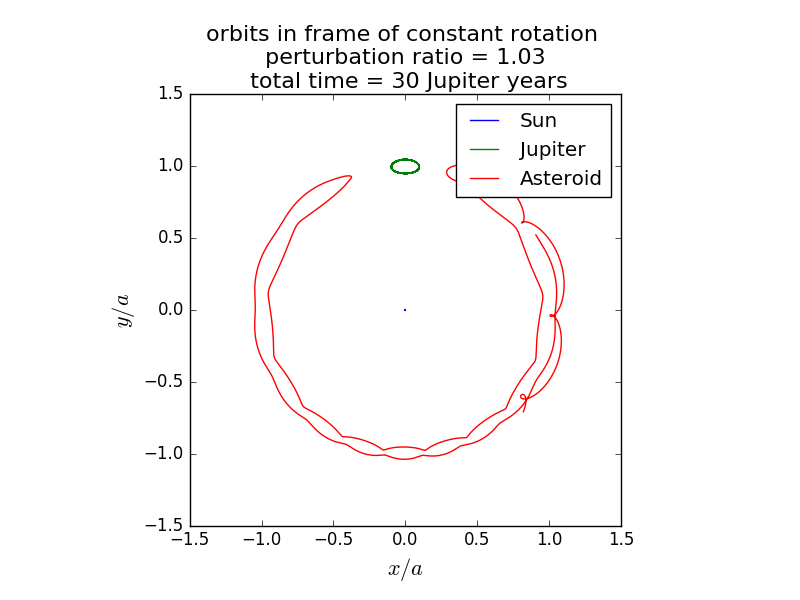
\includegraphics[width = 2.8in]{figure_2_103v_30orbits.png}} 
\subfloat{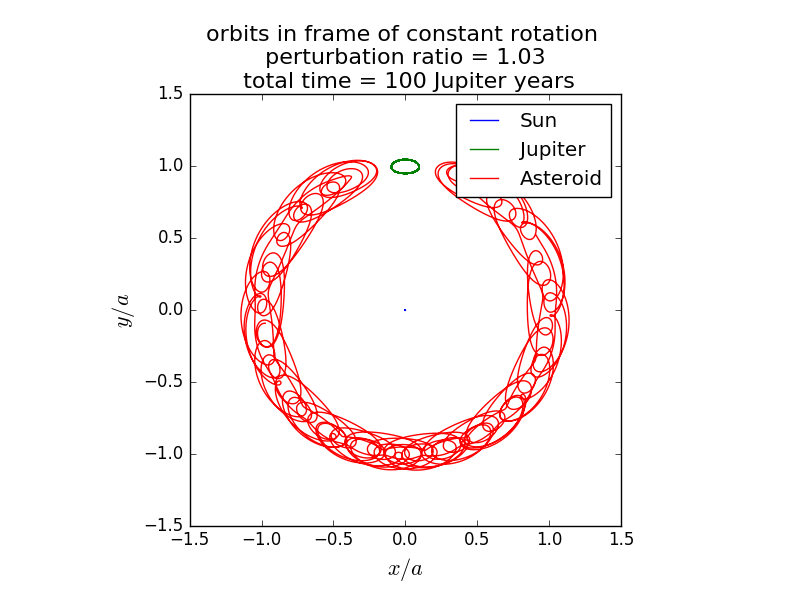
\includegraphics[width = 2.8in]{figure_2_103v_100orbits.png}} \\
\subfloat{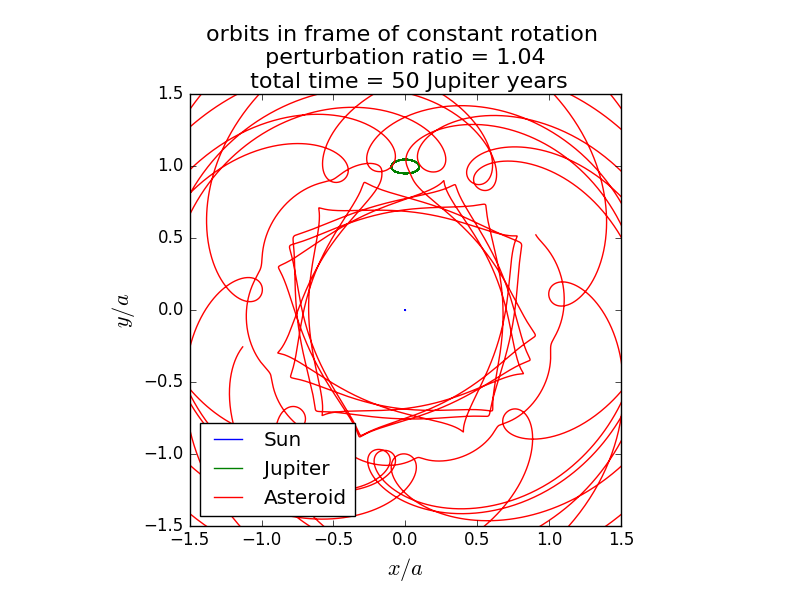
\includegraphics[width = 2.8in]{figure_2_104v_50orbits.png}} 
\subfloat{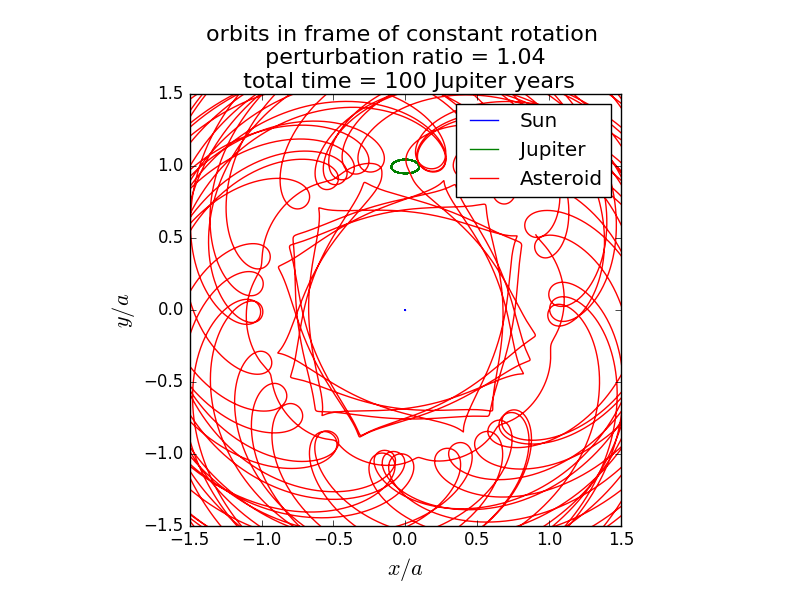
\includegraphics[width = 2.8in]{figure_2_104v_100orbits.png}}

\caption{Orbits of Sun, Jupiter and Trojan asteroid in stationary and constant rotation frames, with different strength of perturbation to Lagrange point initial conditions.}
\label{fig:bigchart}
\end{figure}

Looking at Figure \ref{fig:bigchart} from top to bottom, we can see that, with increasing perturbation ratio to initial velocity (and hence angular velocity), the shape of orbit of asteroid changes from being kidney-bean shaped (perturbation ratio = 1.01 and 1.02) to horse-shoe shaped (ratio = 1.03) and eventually the asteroid escapes from Lagrangian point (ratio = 1.04).

Looking at Figure \ref{fig:bigchart} from left to right, we can see that, the orbit of asteroid does not repeat itself after each cycle. Over long time the trajectory can cover the entire space within the kidney-bean or horse-shoe shape.


\begin{figure}[H]
\centering
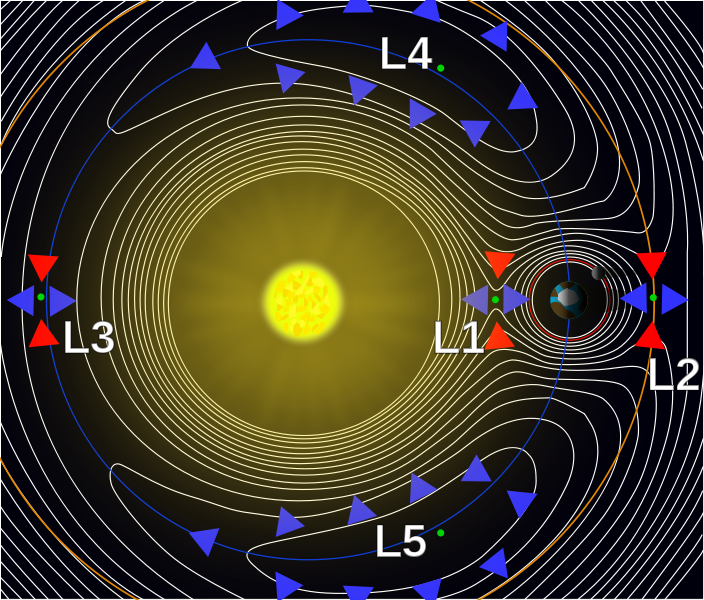
\includegraphics[width=4in]{704px-Lagrange_points2.png}
\caption{A contour plot of the effective potential due to gravity and the centrifugal force of a two-body system in a rotating frame of reference. The arrows indicate the gradients of the potential around the five Lagrange points-downhill toward them (red) or away from them (blue). Counterintuitively, the L4 and L5 points are the high points of the potential. At these points themselves gravity and centrifugal forces are balanced by Coriolis force.}
\label{fig:potential}
\end{figure}


\begin{figure}[H]
\centering
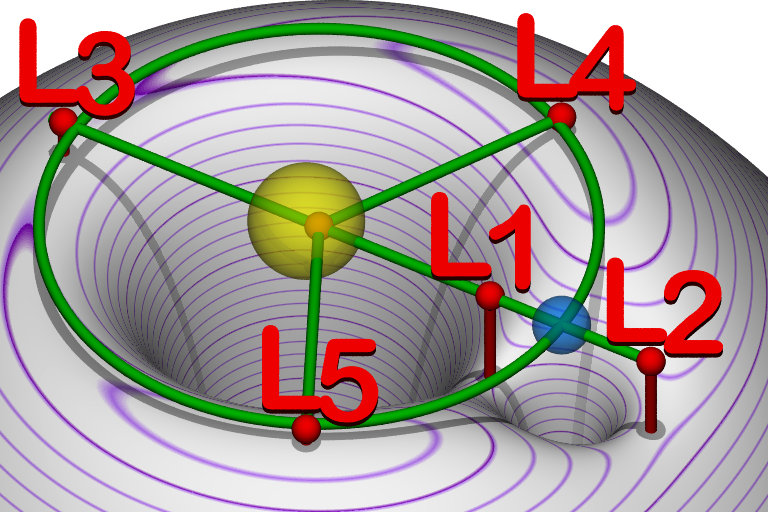
\includegraphics[width=4in]{768px-Lagrangian_points_equipotential}
\caption{Visualization of the relationship between the Lagrangian points (red) of a planet (blue) orbiting a star (yellow) anti-clockwise, and the effective potential in the plane containing the orbit (grey rubber-sheet model with purple contours of equal potential).}
\label{fig:potential2}
\end{figure}


In the rotating frame of constant angular frequency, the asteroid will experience gravitational attraction, centrifugal force, as well as Coriolis force. Because Coriolis force is perpendicular to velocity, it will not affect the energy. Therefore, the effective potential is due to gravity and centrifugal force only (see Figure \ref{fig:potential} and \ref{fig:potential2}). Counterintuitively, Lagrangian points L4 and L5 are at local maxima instead of local minima of effective potential. However, Coriolis force will always act in opposite direction to keep the asteroid close to the contour of effective potential. This is the explanation of the stability of Trojan points, as well as the kidney-bean or horse-shoe shape of the trajectory.


\begin{figure}[H]
\centering
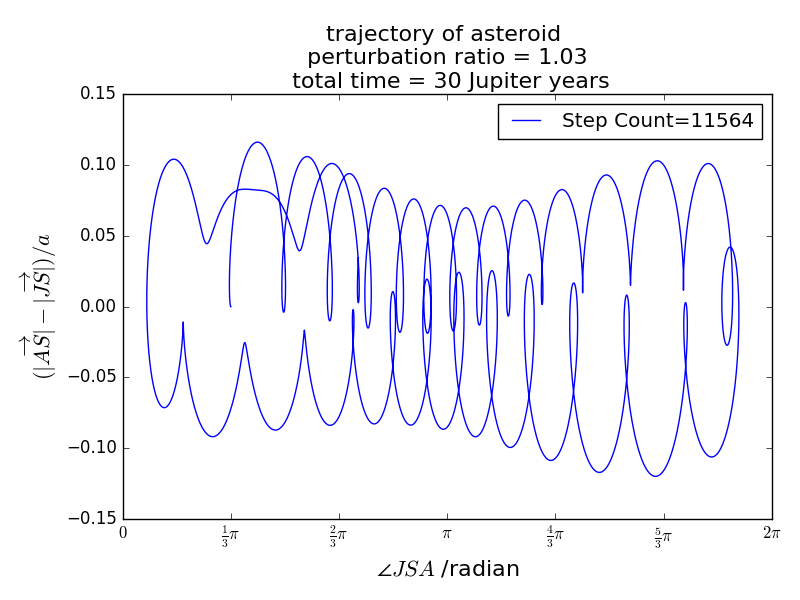
\includegraphics[width=5.5in]{figure_4_103v_30orbits.png}
\caption{Trajectory of Trojan asteroid in 30 Jupiter years, with perturbation ratio 1.03.}
\label{fig:figure_4_103v_30orbits}
\end{figure}

Examining Figure \ref{fig:figure_4_103v_30orbits} closely we can see that, when $|\overrightarrow{AS}| > |\overrightarrow{JS}|$ (centrifugal force greater than gravity), the fact that asteroid moving in clockwise direction induces a inward Coriolis force to balance the difference. When $|\overrightarrow{AS}| < |\overrightarrow{JS}|$ (centrifugal force smaller than gravity), the asteroid moves in counter-clockwise direction so that the Coriolis force balances the difference and keeps the asteroid in stable orbit.

\section{Animations}
This project report includes animations of motions of Sun, Jupiter and Trojan asteroid, in three frames of reference and with different perturbation ratios. Animations are available in GitHub repository (url: \url{https://github.com/nyu-compphys-2016/project-sinochen1992}).  The repository also includes orbit plots that are not included in 'Results and Discussion' section.

\section{Acknowledgements}
Many thanks to teaching assistant Geoffrey Ryan for the helpful discussion on this project and for the numerous support throughout the semester. Without whom I would not have learnt computational physics quickly nor would I get interested in computational physics.

\section{References}
\begin{itemize}
\item Wikipedia
\item 'Computational Physics' textbook by Mark Newman 
\end{itemize}

\end{document}
